\section{The Tutamen Platform}
\label{sec:tutamen}

\subsection{Architecture}

The Tutamen Secret Storage platform has three main components:

\begin{packed_desc}
\item[Access Control Servers (ACS):] The systems responsible for
  storing and enforcing secret access control requirements and for
  authenticating clients making requests.
\item[Storage Servers (SS):] The systems responsible for storing
  secrets (or parts of secrets).
\item[Tutamen Applications (TA):] The systems leveraging the Tutamen
  platform to store and retrieve secrets.
\end{packed_desc}

In general, Tutamen communication occurs between applications and both
types of servers. Tutamen servers do not generally communicates with
each other directly -- with the one exception of storage servers
needing to download the public signing keys from each of the access
control servers with which they interact. All communication in Tutamen
takes place via HTTPS connections - and in some cases leverage mutual
TLS to require both client and server authentication.

Both access control and storage servers are designed to be used
individually or in sets. E.g. An application may store their secret
on a single storage server and delegate access control to a single
access control server, or the application may shard its secret across
multiple storage servers and delegate access control to multiple
access control servers, or any combination thereof. By separating the
access control duties from the secret storage duties, Tutamen offers
the end-user a high degree of flexibility to implement a range of
redundancy and trust requirements.

\subsubsection{Access Control Servers}

The Tutamen Access Control Servers are responsible with authenticating
Tutamen requests as well as storing and enforcing all access control
requirements. Access Control servers expose a number of core data
structures that reflect that manner in which they
operate. Figure~\ref{fig:tutamen:acstructs} shows these structures.

\begin{figure}[th]
  \centering
  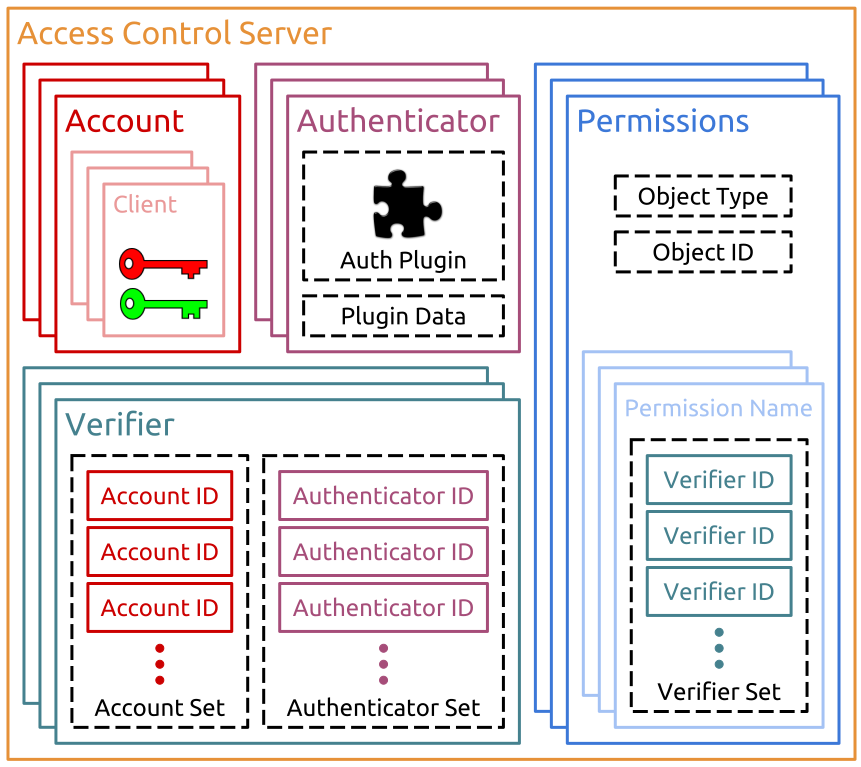
\includegraphics[width=\columnwidth]{./figs/pdf/tutamen-datastructures-ac.pdf}
  \caption{Access Control Server Data Structures}
  \label{fig:tutamen:acstructs}
\end{figure}

In order to track and control access from specific users - the access
control server uses per-user accounts. These accounts are generally
designed to map to individual end-users, but they can be used to track
any singular entity to which one wishes to assign specific access
control privileges. Accounts thus form the basis of controlling and
sharing access to secrets via Tutamen. Within each account are one or
more clients. While accounts map to logically singular access control
entities, clients map to specific devices that will need to make
Tutamen requests. Each account has one or more clients. For example,
Jane Coworker would have a single account with three clients: one for
her laptop, one for her desktop, and one for her phone.

Each client is associated with a single TLS key-pair used to
authenticate the client to the access control server. The access
control server serves as the Certificate Authority administering these
certificates. When a new client is created it generates a local RSA
key and uses this key to generate an X509 Certificate Signing
Request~\cite{rfc5280}. This request is then sent to the access
control server where it awaits approval from an existing client in the
account. If approved, the CSR is used to generate a signed certificate
that is sent back to the new client for use in future access control
server communication. To facilitate bootstrapping new accounts, client
CSRs are also generated and sent with each new account request. These
are atomically approved and associated with the new account --
i.e. the initial client is created in tandem with a new account -- all
subsequent clients are then approved by previously approved clients.

While accounts and clients are used to identify specific
users/entities -- the Tutamen access control server also has
authenticators. Authenticators are modular mechanism used to implement
access control requirements beyond granting access on the basis of
accounts. For example, authenticators can support plugins to perform
additional contextual authentication requirements such as only
allowing access during specific times of day or from requests
originating from specific IP addresses. Authenticators can also be
used to implement out-of-band authentication mechanisms such as
confirming approval for a specific request from a user via text
message or otherwise interfacing with external services to gain
approval.

Accounts and authenticators are combined via verifiers. A verifier
consist of a set of accounts and a set of authenticators. In order to
satisfy a verifier a request must originate from a client in ONE of
the listed accounts and must satisfy ALL of the listed authenticators
plugins. A verifier may contain no Authenticators, in which case
authorization is granted solely on the basis of accounts.

The final component of the Tutamen access control specification are
permission groups. Each permission group corresponds to a specific
object (identified via the combination of an object type and an object
ID) within the Tutamen ecosystem. A permission groups contains one or
more permissions - each corresponding to a specific class of actions
that can be preformed on the corresponding object. Each permission
contains a set of verifiers. In order to be granted a given permission
a request must satisfy at least one of the verifiers in this set.

\subsubsection{Example}

\subsection{Security and Trust}

\subsection{Implementation}

%%  LocalWords:  Tutamen ACS HTTPS CSR CSRs Authenticators verifiers
%%  LocalWords:  authenticators
